\subsubsection{Authentication : Register New User}
Administrators and general users will already be registered on UPRM and their details will be stored on the LDAP authentication database.\\ \\
Third party users should be able to register with UPRM to gain access to the system. The details of such a user will be stored in the UPRM database.\\ \\
\textbf{Pre-Conditions}
\begin{itemize}
	\item The user should provide the following information for registration:
	\begin{itemize}
		\item Name,
		\item Surname,
		\item Username,
		\item Email and
		\item Password \\
	\end{itemize}
\end{itemize}
\textbf{Post-Conditions}
\begin{itemize}
	\item User now has access to UPRM.
	\item User details is stored in the UPRM database.\\
\end{itemize}
\textbf{Register New User Use Case Diagram:}\\
\centerline{\fbox{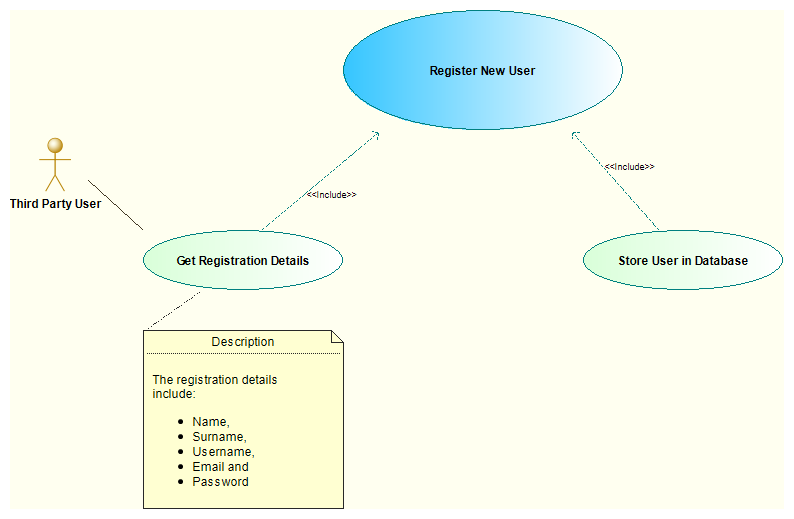
\includegraphics[width=\linewidth]{auth/RegisterNewUser}}}
\subsubsection{Authentication : Login}
Users should be able to login to UPRM.\\
Administrators and General User should be authenticated using LDAP. \\
Third party users should be authenticated using the UPRM database.\\ \\
\textbf{Pre-Conditions}
\begin{itemize}
	\item User should provide the correct username and password.
	\item After receiving the one-time pin the user should provide the system with the correct one-time pin.\\
\end{itemize}
\textbf{Post-Conditions}
\begin{itemize}
	\item If the login was successful,
		\begin{itemize}
			\item a user session should be created and stored.
			\item the user will gain access to UPRM with his/hers specific rights and privileges.
		\end{itemize} 
	\item If the login was not successful,
			\begin{itemize}
				\item the user should be notified of the error that caused the login to be unsuccessful.
				\item the user should have up to 5 tries to login, after which the account will be locked. An administrator should be contacted to unlock the account. \\
			\end{itemize} 
\end{itemize}
\textbf{Login Use Case Diagram:}\\
\centerline{\fbox{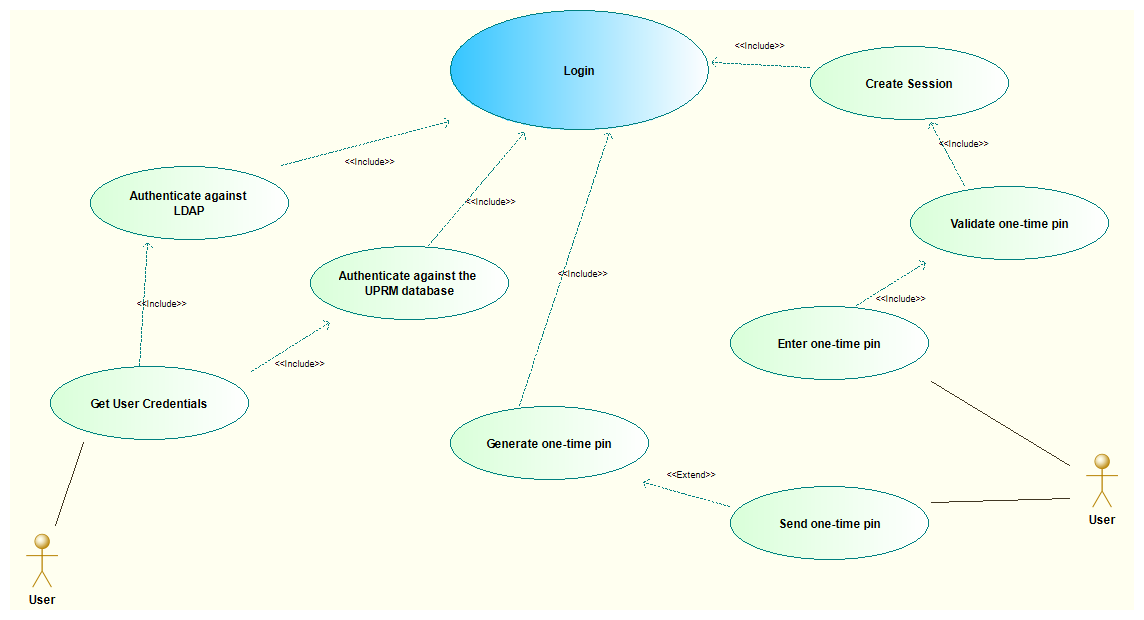
\includegraphics[width=\linewidth]{auth/Login}}}

\subsubsection{Authentication : Logout}
Users should be able to logout of UPRM.\\ \\
\textbf{Pre-Conditions}
\begin{itemize}
	\item User should be logged into UPRM.
	\item A user session should exist.\\
\end{itemize}
\textbf{Post-Conditions}
\begin{itemize}
	\item User not logged into UPRM anymore.
	\item The user session should be removed.\\
\end{itemize}
\textbf{Logout Use Case Diagram:}\\
\centerline{\fbox{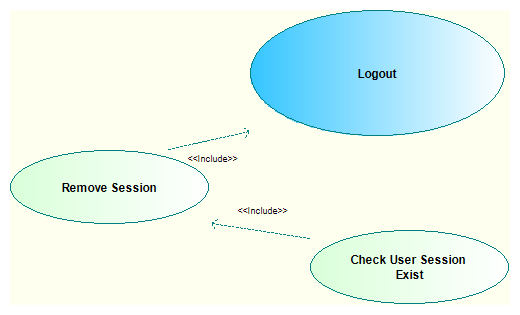
\includegraphics[scale=0.8]{auth/Logout}}}
